% !TEX root =  ../supplementary.tex
\section{Joint Model for the PRIAS Dataset Used in Simulation Study}
\label{sec:param_estimates_jm_fit_prias}
\subsection{Dataset}
In this work we reused a joint model we previously fitted to the PRIAS dataset~\citep{tomer2019personalized,tomer2020webapp}. The PRIAS database is not openly accessible. However, access to the database can be requested on the basis of a study proposal approved by the PRIAS steering committee. The website of the PRIAS program is \url{www.prias-project.org}. For sake of completeness and reproducibility of results we have presented the PRIAS based model's definition and parameter estimates below. Figure~\ref{fig:npmle_plot} shows the cumulative-risk of progression over the follow-up period.

%\begin{table}
%\small
%\centering
%\caption{\textbf{Summary of the PRIAS dataset~\citep{tomer2020webapp}}. The primary event of interest is cancer progression (increase in biopsy Gleason grade group from grade group~1~to~2 or higher). Abbreviations: PSA is prostate-specific antigen; DRE is digital rectal examination, with level T1c~\citep{schroder1992tnm} indicating a clinically inapparent tumor which is not palpable or visible by imaging, whereas tumors with $\mbox{DRE} > \mbox{T1c}$ are palpable; IQR is interquartile range.}
%\label{table:prias_summary}
%\begin{tabular}{lr}
%\hline
%\hline
%\textbf{Characteristic} &  \textbf{Value}\\
%\hline
%Total patients &  7813\\
%\textit{progression (primary event)}  & 1134\\
%Treatment  &  2250\\
%Watchful waiting   & 334\\
%Lost to follow-up   & 203\\
%Discontinued on request   & 46\\
%Death (other)   & 95\\
%Death (prostate cancer)   & 2\\
%\hline
%Total DRE measurements & 37326 \\
%Total PSA measurements  & 67578\\
%Total biopsies & 15686\\
%\hline
%Median follow-up period per patient (years)   &  1.8 (IQR: 0.9--4.0)\\
%Median age at diagnosis (years)   & 66 (IQR: 61--71)\\
%Median PSA (ng/mL) & 5.7 (IQR: 4.1--7.7)\\
%$\mbox{DRE} = \mbox{T1c}$ (\%)  & 34883/37326 (94\%) \\
%\hline
%Median number of PSA per patient   &  6 (IQR: 4--12)\\
%Median number of DRE per patient & 4 (IQR: 2--7)\\
%Median number of biopsies per patient  &  2 (IQR: 1--2)\\
%\hline
%\end{tabular}
%\end{table}
 
\begin{figure}
\captionsetup{justification=justified}
\centerline{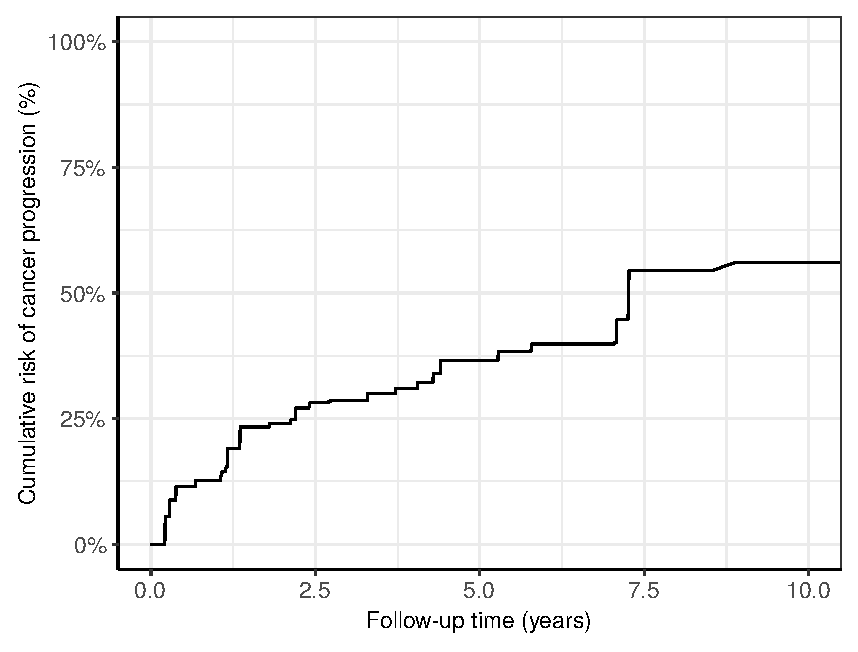
\includegraphics[width=\columnwidth]{images/npmle_plot.eps}}
\caption{\textbf{Estimated cumulative-risk of cancer progression~\citep{tomer2020webapp}} for patients in the Prostate Cancer Research International Active Surveillance (PRIAS) dataset. Nearly 50\% patients (\textit{slow progressing}) do not progress in the ten year follow-up period. Cumulative risk is estimated using nonparametric maximum likelihood estimation \citep{turnbull1976empirical}, to account for interval censored progression times observed in the PRIAS dataset. Censoring includes death, removal from surveillance on the basis of observed longitudinal data, and patient dropout.}
\label{fig:npmle_plot}
\end{figure}

\subsection{Model Specification}
Let $T_i^*$ denote the true progression time of the ${i\mbox{-th}}$ patient included in PRIAS. Since biopsies are conducted periodically, $T_i^*$ is observed with interval censoring ${l_i < T_i^* \leq r_i}$. When progression is observed for the patient at his latest biopsy time $r_i$, then $l_i$ denotes the time of the second latest biopsy. Otherwise, $l_i$ denotes the time of the latest biopsy and ${r_i=\infty}$. Let $\boldsymbol{y}_{di}$ and $\boldsymbol{y}_{pi}$ denote his observed DRE (digital rectal examination) and PSA (prostate-specific antigen) longitudinal measurements, respectively. The observed data of all $n$ patients is denoted by ${\mathcal{D}_n = \{l_i, r_i, \boldsymbol{y}_{di}, \boldsymbol{y}_{pi}; i = 1, \ldots, n\}}$.

The patient-specific DRE and PSA measurements over time are modeled using a bivariate generalized linear mixed effects sub-model. The sub-model for DRE is given by:
\begin{equation}
\label{eq:long_model_dre}
\begin{split}
    \mbox{logit} \big[\mbox{Pr}\{y_{di}(t) > \mbox{T1c}\}\big] &= \beta_{0d} + b_{0di} + (\beta_{1d} + b_{1di}) t\\
    &+ \beta_{2d} (\mbox{Age}_i-65) + \beta_{3d} (\mbox{Age}_i-65)^2
    \end{split}
\end{equation}
where, $t$ denotes the follow-up visit time, and $\mbox{Age}_i$ is the age of the ${i\mbox{-th}}$ patient at the time of inclusion in AS. The fixed effect parameters are denoted by ${\{\beta_{0d}, \ldots, \beta_{3d}\}}$, and ${\{b_{0di}, b_{1di}\}}$ are the patient specific random effects. With this definition, we assume that the patient-specific log odds of obtaining a DRE measurement larger than T1c (palpable tumor) remain linear over time. 

The mixed effects sub-model for PSA is given by:
\begin{equation}
\label{eq:long_model_psa}
\begin{split}
    \log_2 \big\{y_{pi}(t) + 1\big\} &= m_{pi}(t) + \varepsilon_{pi}(t),\\
    m_{pi}(t) &= \beta_{0p} + b_{0pi} + \sum_{k=1}^3 (\beta_{kp} + b_{kpi})  B_k(t,\mathcal{K})\\ 
    &+ \beta_{4p} (\mbox{Age}_i-65) + \beta_{5p} (\mbox{Age}_i-65)^2,
    \end{split}
\end{equation}
where, $m_{pi}(t)$ denotes the underlying measurement error free value of $\log_2 (\mbox{PSA} + 1)$ transformed \citep{pearson1994mixed,lin2000latent} measurements at time $t$. We model it non-linearly over time using B-splines \citep{de1978practical}. To this end, the B-spline basis function $B_k(t, \mathcal{K})$ has 3 internal knots at $\mathcal{K} = \{0.75, 2.12\}$ years (33-rd and 66-th percentile of observed follow-up times), and boundary knots at 0 and 6.4 years (95-th percentile of the observed follow-up times). The fixed effect parameters are denoted by ${\{\beta_{0p},\ldots,\beta_{5p}\}}$, and ${\{b_{0pi}, \ldots, b_{3pi}\}}$ are the patient specific random effects. The error $\varepsilon_{pi}(t)$ is assumed to be t-distributed with three degrees of freedom~\citep{tomer2019personalized} and scale $\sigma$, and is independent of the random effects. 

To account for the correlation between the DRE and PSA measurements of a patient, link their corresponding random effects are linked. Specifically, the complete vector of random effects ${\boldsymbol{b}_i = (b_{0di}, b_{1di}, b_{0pi}, \ldots, b_{3pi})^\top}$ is assumed to follow a multivariate normal distribution with mean zero and variance-covariance matrix $\boldsymbol{W}$.

To model the impact of DRE and PSA measurements on the risk of progression, the joint model uses a relative risk sub-model. More specifically, the hazard of progression $h_i(t)$ at a time $t$ is given by:
\begin{equation}
\label{eq:rel_risk_model}
\begin{split}
    h_i(t) &= h_0(t) \exp\Big(\gamma_1 (\mbox{Age}_i-65) + \gamma_2 (\mbox{Age}_i-65)^2\\
    &+\alpha_{1d} \mbox{logit} \big[\mbox{Pr}\{y_{di}(t) > \mbox{T1c}\}\big]+ \alpha_{1p} m_{pi}(t) + \alpha_{2p} \frac{\partial m_{pi}(t)}{\partial {t}}\Big),
    \end{split}
\end{equation}
where, $\gamma_1, \gamma_2$ are the parameters for the effect of age. The parameter $\alpha_{1d}$ models the impact of log odds of obtaining a $\mbox{DRE} > \mbox{T1c}$ on the hazard of progression. The impact of PSA on the hazard of progression is modeled in two ways: a) the impact of the error free underlying PSA value $m_{pi}(t)$, and b) the impact of the underlying PSA velocity $\partial m_{pi}(t)/\partial {t}$. The corresponding parameters are $\alpha_{1p}$ and $\alpha_{2p}$, respectively. Lastly, $h_0(t)$ is the baseline hazard at time t, and is modeled flexibly using P-splines \citep{eilers1996flexible}.

\subsection{Parameter Estimates}
The posterior parameter estimates for the PRIAS based joint model are shown in \ref{tab:DRE_long} (longitudinal sub-model for DRE outcome), \ref{tab:PSA_long} (longitudinal sub-model for PSA outcome) and \ref{tab:DRE_PSA_survival} (relative risk sub-model). The parameter estimates for the variance-covariance matrix $\boldsymbol{W}$ from the longitudinal sub-model are shown in the following \ref{tab:D_matrix}:

\begin{table}[!htb]
\begin{center}
\caption{Estimated variance-covariance matrix $\boldsymbol{W}$ of the random effects ${\boldsymbol{b}=(b_{0d},b_{1d},b_{0p}, b_{1p}, b_{2p}, b_{3p})}$ from the joint model fitted to the PRIAS dataset.}
\label{tab:D_matrix}
\begin{tabular}{lrrrrrr}
\hline
\hline
Random Effects    & $b_{0d}$    & $b_{1d}$    & $b_{0p}$    & $b_{1p}$   & $b_{2p}$   & $b_{3p}$ \\
\hline
$b_{0d}$ & 9.233 & -0.183 & -0.213 & 0.082 & 0.058 & 0.023 \\
$b_{1d}$ & -0.183 & 1.259 & 0.091 & 0.079 & 0.145 & 0.109 \\
\hline
$b_{0p}$ & -0.213 & 0.091 & 0.247 & 0.007 & 0.067 & 0.018 \\
$b_{1p}$ & 0.082 & 0.079 & 0.007 & 0.248 & 0.264 & 0.189 \\
$b_{2p}$ & 0.058 & 0.145 & 0.067 & 0.264 & 0.511 & 0.327 \\
$b_{3p}$ & 0.023 & 0.109 & 0.018 & 0.189 & 0.327 & 0.380 \\
\hline
\end{tabular}
\end{center}
\end{table}

\begin{table}[!htb]
\begin{center}
\caption{Estimated mean and 95\% credible interval for the parameters of the longitudinal sub-model~(\ref{eq:long_model_dre}) for the DRE outcome.}
\label{tab:DRE_long}
\begin{tabular}{lrrrr}
\hline
\hline
Variable                         & Mean & Std. Dev & 2.5\%  & 97.5\%   \\
\hline
(Intercept)                      & -4.407 & 0.151 & -4.716 & -4.113 \\
$(\mbox{Age} - 65)$              & 0.057 & 0.009 & 0.039 & 0.075 \\
$(\mbox{Age} - 65)^2$            & -0.002 & 0.001 & -0.004 & 0.000\\
visitTimeYears                   & -1.089 & 0.113 & -1.292 & -0.866 \\
\hline
\end{tabular}
\end{center}
\end{table}

\begin{table}[!htb]
\begin{center}
\caption{Estimated mean and 95\% credible interval for the parameters of the longitudinal sub-model~(\ref{eq:long_model_psa}) for the PSA outcome.}
\label{tab:PSA_long}
\begin{tabular}{lrrrr}
\hline
\hline
Variable                         & Mean & Std. Dev & 2.5\%  & 97.5\% \\
\hline
(Intercept) & 2.687 & 0.007 & 2.674 & 2.701 \\
$(\mbox{Age} - 65)$ & 0.008 & 0.001 & 0.006 & 0.010 \\
$(\mbox{Age} - 65)^2$ & -0.001 & 0.000 & -0.001 & 0.000 \\
Spline: [0.00, 0.75] years & 0.199 & 0.009 & 0.181 & 0.217 \\
Spline: [0.75, 2.12] years & 0.293 & 0.012 & 0.269 & 0.316 \\
Spline: [2.12, 6.4] years & 0.379 & 0.014 & 0.352 & 0.406\\
$\sigma$ & 0.144 & 0.001 & 0.142 & 0.145\\
\hline
\end{tabular}
\end{center}
\end{table}

%We present plots of observed DRE versus fitted probabilities of obtaining a DRE measurement larger than T1c, for nine randomly selected patients in Figure~\ref{fig:fitted_9subject_dre}. Similarly observed versus fitted PSA profiles for nine randomly selected patients are shown in Figure~\ref{fig:fitted_9subject_psa}. 

%\begin{figure}[!htb]
%\centerline{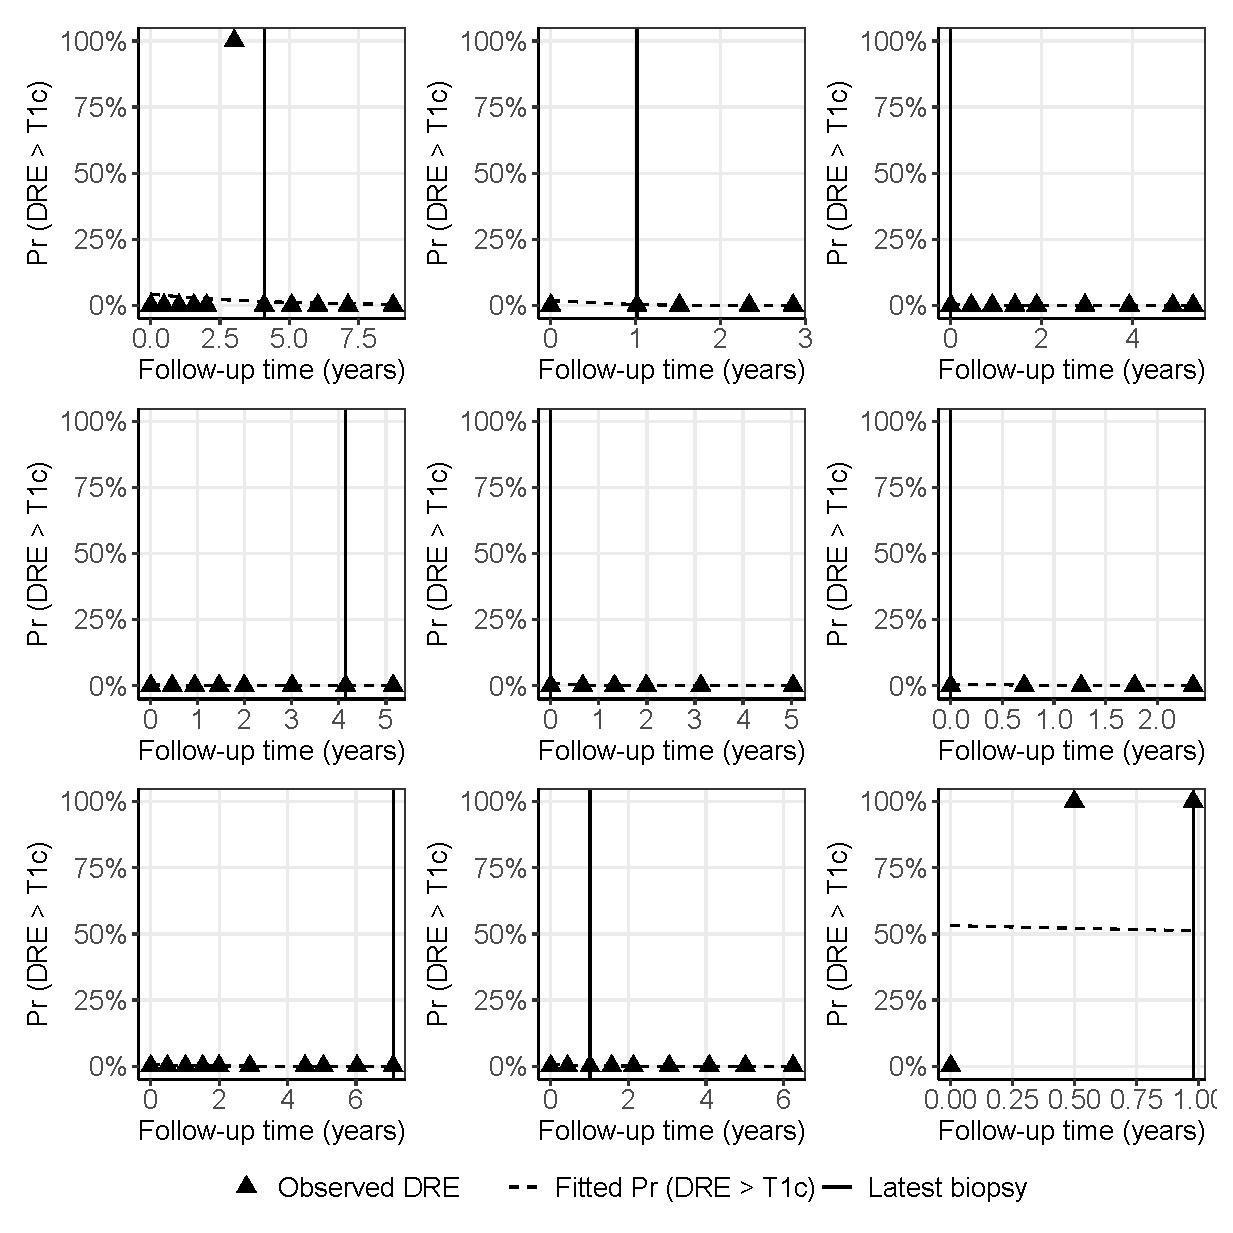
\includegraphics[width=\columnwidth]{images/fitted_9subject_dre.eps}}
%\caption{Observed DRE versus fitted probabilities of obtaining a DRE measurement larger than T1c, for nine randomly selected PRIAS patients. The fitted profiles utilize information from the observed DRE measurements, PSA measurements, and time of the latest biopsy. Observed DRE measurements plotted against 0\% probability are equal to T1c. Observed DRE measurements plotted against 100\% probability are larger than T1c.}
%\label{fig:fitted_9subject_dre}
%\end{figure}

%\begin{figure}[!htb]
%\centerline{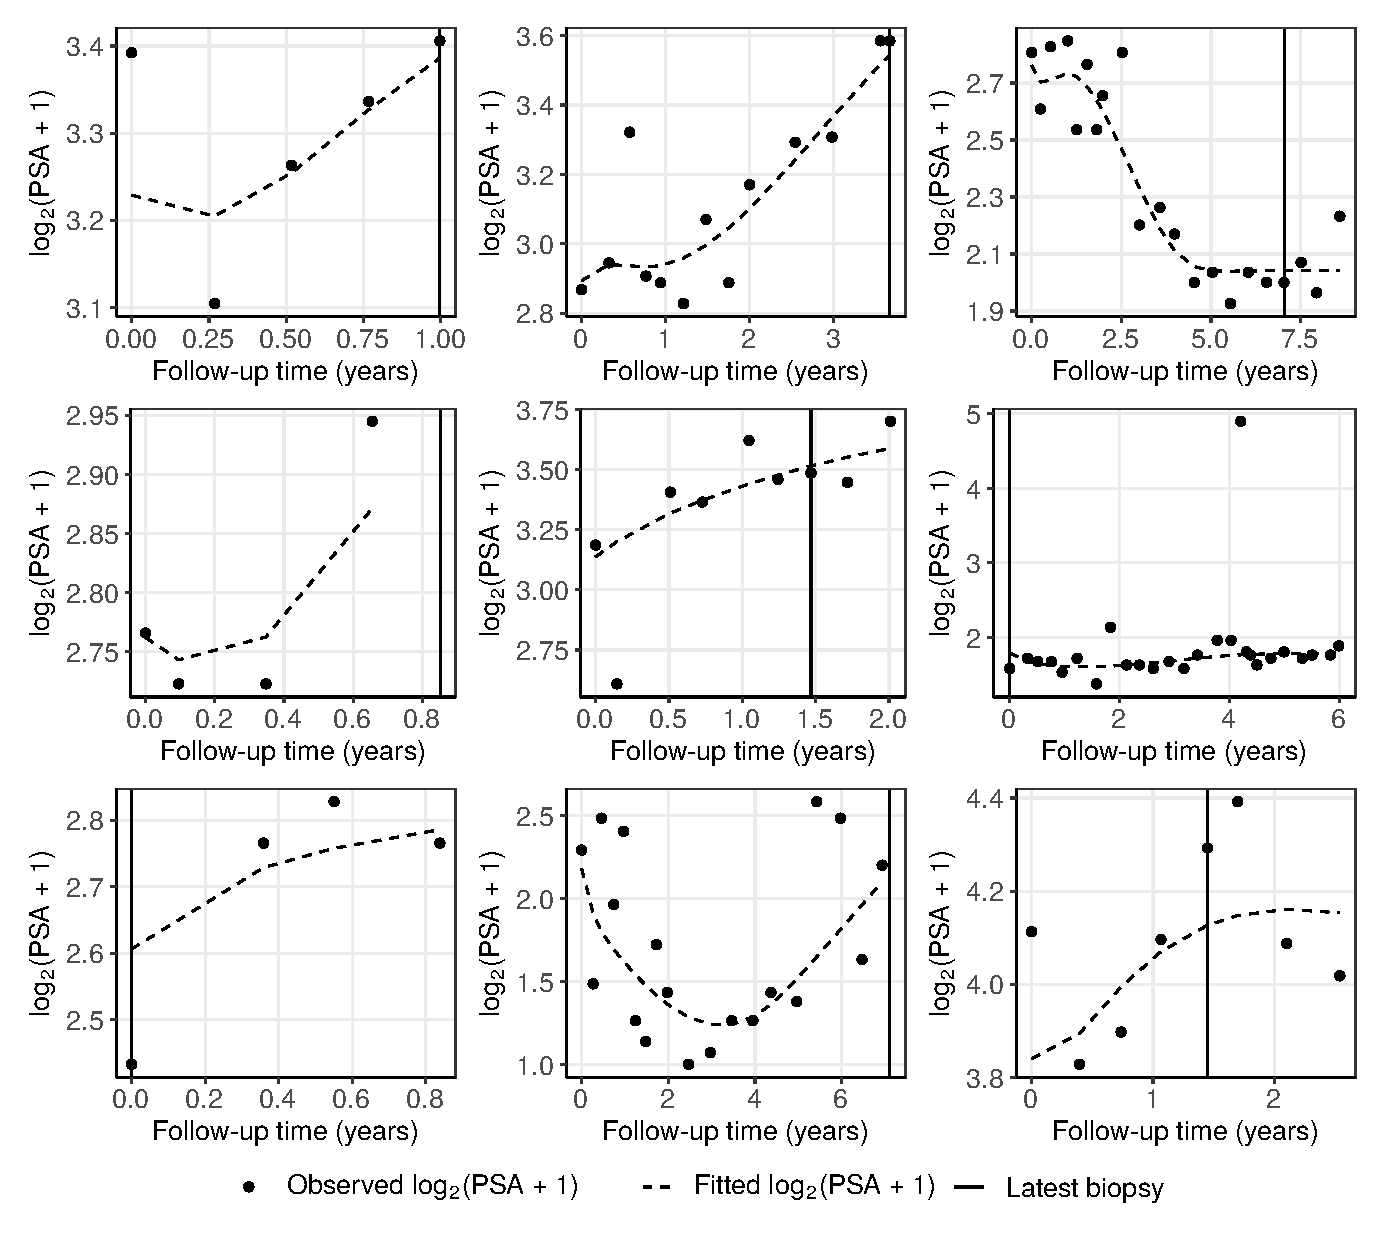
\includegraphics[width=\columnwidth]{images/fitted_9subject_psa.eps}}
%\caption{Fitted versus observed ${\log_2 (\mbox{PSA} + 1)}$ profiles for nine randomly selected PRIAS patients. The fitted profiles utilize information from the observed PSA measurements, DRE measurements, and time of the latest biopsy.}
%\label{fig:fitted_9subject_psa}
%\end{figure}

For the relative risk sub-model~(\ref{eq:rel_risk_model}), the parameter estimates in \ref{tab:DRE_PSA_survival} show that both ${\log_2 (\mbox{PSA} + 1)}$ velocity, and the log odds of having ${\mbox{DRE} > \mbox{T1c}}$  were significantly associated with the hazard of progression.  
\begin{table}[!htb]
\begin{center}
\caption{Estimated mean and 95\% credible interval for the parameters of the relative risk sub-model~(\ref{eq:rel_risk_model}) of the joint model fitted to the PRIAS dataset.}
\label{tab:DRE_PSA_survival}
\begin{tabular}{lrrrr}
\hline
\hline
Variable                      & Mean   & Std. Dev & 2.5\%  & 97.5\% \\
\hline
$(\mbox{Age} - 65)$  & 0.034 & 0.005 & 0.025 & 0.043 \\
$(\mbox{Age} - 65)^2$ & 0.000 & 0.001 & -0.001 & 0.001 \\
$\mbox{logit} \big\{\mbox{Pr}(\mbox{DRE} > \mbox{T1c})\big\}$ & 0.047 & 0.014 & 0.018 & 0.073 \\
Fitted $\log_2 (\mbox{PSA} + 1)$ value  & 0.024 & 0.076 & -0.125 & 0.170\\
Fitted $\log_2 (\mbox{PSA} + 1)$ velocity  & 2.656 & 0.291 & 2.090 & 3.236 \\
\hline
\end{tabular}
\end{center}
\end{table}

As described in~\ref{sec:jointmodel} the baseline hazard of the joint model model utilized a cubic P-spline. The knots of this P-spline were placed at the following time points:
0.000, 0.000, 0.000, 0.000, 0.401, 0.801, 1.202, 1.603, 2.003, 2.404, 2.805, 3.205, 3.606, 4.007, 4.407, 4.808, 5.209, 12.542, 12.542, 12.542, 12.542
The parameters of the fitted spline function are given in~\ref{tab:baseline_hazard}.
\begin{table}[!htb]
\begin{center}
\caption{Estimated parameters of the P-spline function utilized to model the baseline hazard $h_0(t)$ in joint model fitted to the PRIAS dataset. Parameters are named with the prefix `ps' indicating P-spline parameter.}
\label{tab:baseline_hazard}
\begin{tabular}{lrrrrrr}
\hline
\hline
Variable                         & Mean & Std. Dev & 2.5\%  & 97.5\%   \\
\hline
ps1  & -1.091 & 0.535 & -2.286 & -0.235 \\
ps2  & -2.113 & 0.271 & -2.638 & -1.591 \\
ps3  & -2.486 & 0.308 & -3.095 & -1.883 \\
ps4  & -2.083 & 0.311 & -2.740 & -1.483 \\
ps5  & -1.918 & 0.279 & -2.460 & -1.388 \\
ps6  & -2.620 & 0.265 & -3.138 & -2.140 \\
ps7  & -3.169 & 0.303 & -3.796 & -2.580 \\
ps8  & -3.416 & 0.340 & -4.075 & -2.823 \\
ps9  & -3.432 & 0.345 & -4.103 & -2.796 \\
ps10 & -3.223 & 0.352 & -3.997 & -2.573 \\
ps11 & -2.840 & 0.349 & -3.577 & -2.214 \\
ps12 & -2.481 & 0.350 & -3.148 & -1.762 \\
ps13 & -2.540 & 0.352 & -3.206 & -1.840 \\
ps14 & -2.841 & 0.321 & -3.447 & -2.212 \\
ps15 & -3.046 & 0.381 & -3.853 & -2.328 \\
ps16 & -3.113 & 0.701 & -4.533 & -1.796 \\
ps17 & -3.195 & 1.232 & -5.894 & -0.978 \\
\hline
\end{tabular}
\end{center}
\end{table}

Data of the demonstration patient in Figure~5 of the main manuscript is available in~\ref{tab:demo_patient}.

\begin{table}[!htb]
\begin{center}
\caption{Data of the demonstration patient in Figure~5 of the main manuscript. Age of the patient at baseline was 60 years and time of last negative biopsy was 3.5 years. DRE: digital rectal examination.}
\label{tab:demo_patient}
\begin{tabular}{rrrr}
\hline
Visit time (years) & PSA & $\log_2(\mbox{PSA}+1)$ & DRE > T1c\\ 
\hline
0.00 & 5.7 & 2.77 &            1\\
0.30 & 3.2 & 2.09 &           -\\
0.68 & 4.0 & 2.30 &            0\\
0.97 & 4.6 & 2.50 &           -\\
1.15 & 2.9 & 1.92 &            0\\
1.47 & 3.0 & 1.95 &            0\\
1.77 & 3.3 & 2.14 &           -\\
2.23 & 3.5 & 2.12 &            0\\
2.58 & 4.4 & 2.39 &           -\\
3.21 & 6.1 & 2.84 &            0\\
3.86 & 5.9 & 2.81 &           -\\
4.32 & 3.9 & 2.31 &            0\\
5.00 & 4.4 & 2.41 &           -\\
\hline
\end{tabular}   
\end{center}
\end{table}

%It is important to note that since age, ${\log_2 (\mbox{PSA} + 1)}$ value and velocity, and log odds of ${\mbox{DRE} > \mbox{T1c}}$ are all measured on different scales, a comparison between the corresponding parameter estimates is not easy. To this end, in \ref{tab:DRE_PSA_survival_easy}, we present the hazard (of progression) ratio, for an increase in the aforementioned variables from their first to the third quartile. For example, an increase in log odds of DRE > T1c, from -6.650 to -4.356 (fitted first and third quartiles) corresponds to a hazard ratio of 1.402. The interpretation for the rest is similar.

%\begin{table}[!htb]
%\begin{center}
%\caption{Hazard (of progression) ratio and 95\% credible interval (CI), for an increase in the variables of relative risk sub-model, from their first quartile ($\mbox{Q}_1$) to their third quartile ($\mbox{Q}_3$). Except for age, quartiles for all other variables are based on their fitted values obtained from the joint model fitted to the PRIAS dataset.}
%\label{tab:DRE_PSA_survival_easy}
%\begin{tabular}{lrrr}
%\hline
%\hline
%Variable                      & $\mbox{Q}_1$   & $\mbox{Q}_3$ & Hazard ratio [95\% CI] \\
%\hline
%Age & 61 & 71 & 1.402 [1.282, 1.539] \\
%$\mbox{logit} \big\{\mbox{Pr}(\mbox{DRE} > \mbox{T1c})\big\}$ & -8.278 & -5.155 & 1.157 [1.057, 1.255]\\
%$\log_2 (\mbox{PSA} + 1)$ value & 2.362 & 3.076 & 1.017 [0.914, 1.129]\\
%$\log_2 (\mbox{PSA} + 1)$ velocity & -0.033 & 0.145 & 1.603 [1.450, 1.778]\\
%\hline
%\end{tabular}
%\end{center}
%\end{table}

%\clearpage

%\subsection{Assumption of t-distributed (df=3) Error Terms}
%\label{subsec:t-dist-assumption}
%With regards to the choice of the distribution for the error term $\varepsilon_p$ for the PSA measurements (see~\ref{eq:long_model_psa}), we attempted fitting multiple joint models differing in error distribution, namely t-distribution with three, and four degrees of freedom, and a normal distribution for the error term. However, the model assumption for the error term were best met by the model with t-distribution having three degrees of freedom. The quantile-quantile plot of subject-specific residuals for the corresponding model in Panel~A of Figure~\ref{fig:qqplot}, shows that the assumption of t-distributed (df=3) errors is reasonably met by the fitted model. 

%\begin{figure}[!htb]
%\centerline{\includegraphics[width=\columnwidth]{images/qqplot.eps}}
%\caption{Quantile-quantile plot of subject-specific residuals from the joint models fitted to the PRIAS dataset. \textbf{Panel A}: model assuming a t-distribution (df=3) for the error term $\varepsilon_p$. \textbf{Panel B}: model assuming a normal distribution for the error term $\varepsilon_p$.}
%\label{fig:qqplot}
%\end{figure}

%\clearpage
We present the predictive performance of the PRIAS based joint model using the area under the receiver operating characteristic curve or AUC (measure of discrimination), and the mean absolute prediction error (MAPE) in~\ref{tab:AUC_PE}. In a joint model these are calculated in a time-dependent manner~\citep{landmarking2017}. More specifically, given the time of latest biopsy $t$, and history of longitudinal data up to time $s$, we are interested in a medically relevant time frame $(t, s]$, within which the occurrence of progression is of interest, e.g., 1 year in prostate cancer. That is, $s = t+1$. The AUC and MAPE at every six months (schedule of PSA/DRE measurement follow-up in PRIAS) between year one and year six (roughly the 95-percentile of observed follow-up times) are presented in~\ref{tab:AUC_PE}.

\begin{table}[!htb]
\begin{center}
\caption{Follow-up time dependent, area under the receiver operating characteristic curves (AUC), and mean absolute prediction error (MAPE), with 95\% confidence interval in brackets.}
\label{tab:AUC_PE}
\begin{tabular}{r|r|r}
\hline
\hline
Follow-up period (years) & AUC (95\% CI) & MAPE (95\%CI)\\ 
\hline
0.0 to 1.0 & 0.658 [0.620, 0.693] & 0.234 [0.229, 0.240]\\
0.5 to 1.5 & 0.648 [0.631, 0.663] & 0.220 [0.213, 0.226]\\
1.0 to 2.0 & 0.624 [0.600, 0.644] & 0.151 [0.147, 0.155]\\
1.5 to 2.5 & 0.649 [0.604, 0.704] & 0.127 [0.118, 0.134]\\
2.0 to 3.0 & 0.683 [0.629, 0.729] & 0.134 [0.121, 0.143]\\
2.5 to 3.5 & 0.681 [0.604, 0.739] & 0.115 [0.105, 0.128]\\
3.0 to 4.0 & 0.647 [0.600, 0.710] & 0.079 [0.073, 0.087]\\
3.5 to 4.5 & 0.630 [0.583, 0.668] & 0.095 [0.089, 0.101]\\
4.0 to 5.0 & 0.614 [0.557, 0.659] & 0.104 [0.098, 0.111]\\
4.5 to 5.5 & 0.615 [0.541, 0.702] & 0.101 [0.088, 0.114]\\
5.0 to 6.0 & 0.617 [0.550, 0.713] & 0.102 [0.086, 0.121]\\
\hline
\end{tabular}	
\end{center}
\end{table}